% !TEX encoding = UTF-8
% !TEX TS-program = pdflatex
% !TEX root = computabilità e algoritmi.tex
% !TEX spellcheck = it-IT
\subsection{Codice del merge parallelo}\label{codice-del-merge-parallelo}

Ci sarebbe prima il codice della ricerca binaria, ma è quella classica
sequenziale e che ritorna l'indice dell'elemento in tempo $O(\log n)$

\begin{breakablealgorithm}
	\caption{\textsc{P-Merge}: merge di due array parallelizzato}
	\begin{algorithmic}[1]
\Function{P-Merge}{$T, p_1, r_1, p_2, r_2, A, p_e$}
    \State $n_1 \gets r_1 - p_1 +1$
    \State $n_2 \gets r_2 - p_2 +1$
    \If{$n_1 < n_2$}
        \State inverti le due parti in modo che $n_1 \geq n_2$
    \EndIf
    \If{$n_1 = 0$}
        \State \Return
    \EndIf
    \State $q_1 \gets \lfloor (p_1 + r_1) / 2 \rfloor$ \Comment{Elemento mediano della prima parte}
    \State $q_2 \gets \textsc{Binary-Search}(T[q_1], T, p_2, r_2)$
    \State $q_3 \gets p_3 + (q_1 - p_1) + (q_2 - p_2)$ 
    \State $A[q_3] \gets T[q_1]$
    \State \textbf{spawn } \textsc{P-Merge}$(T, p_1, q_1 -1, p_2, q_2 -1, A, p_3)$ \Comment{Unisce i valori $\leq x$}
    \State \textsc{P-Merge}$(T, q_1 +1, r_1, q_2, r_2, A, q_3+1)$
    \State \textbf{sync}
\EndFunction
\end{algorithmic}
\end{breakablealgorithm}

\subsubsection{Analisi della complessità}\label{analisi-della-complessituxe0}

La durata $PM_\infty(n)$ del merge è data da una costante per i vari calcoli dell'indice, più un tempo logaritmico per la ricerca binaria, più il tempo delle due chiamate che vengono fatte in parallelo.

La durate delle chiamate parallele dipende dal blocco più grande, ma che dimensione ha?

Ogni chiamata, nella peggiore delle ipotesi viene fatta su $n_1/2 + n_2$ elementi, $n_2$ deriva dal fatto che gli elementi della seconda parte dell'array possono essere tutti minori di $x$ o tutti maggiori uguali.

$$\frac{n_1}{2} +n_2 = \frac{n_1}{2} + \frac{n_2}{2} + \frac{n_2}{2} \leq \frac{n}{2} + \frac{n}{4} = \frac{3n}{4}$$

Si ha quindi che

$$
PM_\infty(n) \leq PM_\infty(\frac{3}{4}n) + O(\log n) = O(\log^2 n)
$$

Per quanto riguarda il lavoro si ha

$$
PM_1(n) = PM_1(\alpha n) + PM_1( (1-\alpha) n) + O(\log n)
$$

perché è dato dalla somma del lavoro delle due parti parallele, più il lavoro necessario per la ricerca binaria.

Per quanto riguarda $\alpha$ si ha che è nel range $1/4 \leq \alpha \leq 3/4$.

Risparmiando i conti, il lavoro finale è dato da

$$
PM_1(n) \leq c_1 - c_2 \log (n) = \Theta (n)
$$

Il parallelismo di questo algoritmo risulta essere buono, perché

$$
\frac{PM_1}{PM_\infty} = \Theta \Big(\frac{n}{\log^2 n}\Big)
$$

e si ottiene uno speedup quasi lineare già per $n$ maggiore di 10.

\subsection{Merge Sort parallelo v2}\label{merge-sort-parallelo-v2}

\begin{breakablealgorithm}
	\caption{\textsc{P-Merge-Sort}: merge sort parallelizzato bene}
	\begin{algorithmic}[1]
\Function{P-Merge-Sort}{$A,p,r, B, S$}
\State $n \gets r - p +1$
\If{$n = 1$}
    \State \Return
\EndIf 
\If{$p < r$}
    \State $T[1 \ldots n] $ nuovo array
    \State $q \gets floor(p+r/2)$
    \State $q' \gets q - p +1$
    \State \textbf{spawn } \textsc{P-Merge-Sort}$(A,p,q, T, 1)$
    \State \textsc{P-Merge-Sort}$(A,q+1,r, T, q'+1)$
    \State \textbf{sync}
    \State \textsc{P-Merge}$(T, 1, q', q'+1, n, B, s)$
\EndIf
\EndFunction
\end{algorithmic}
\end{breakablealgorithm}

Questa versione modificata riceve come parametro anche un'array dove mettere gli elementi una volta ordinati ed esegue le chiamate ricorsive in parallelo.

La differenza sta che una volta sincronizzate le due chiamate, il merge viene fatto con la procedura parallela.

Il lavoro di questa versione è

$$
MS_1(n) = 2 MS_1(n/2) + \Theta(n) = \Theta (n \log n)
$$

che è lo stesso della versione precedente.

La durata invece è

\begin{align*}
MS_\infty (n) &= MS_\infty (n/2) + \Theta(\log^2 n) \\
              &=\Theta (\log^3 n)
\end{align*}

ovvero la durata di una delle due chiamate ricorsive parallele, che tanto sono uguali perché l'array viene diviso a metà, più la durata dell merge ricorsivo.

Anche in questo caso il parallelismo risulta essere

$$
O(\frac{n}{\log^2 n})
$$

\section{P-Scan}\label{p-scan}

Si ha a disposizione un'array e una certa operazione associativa da effettuare sugli elementi dell'array, come la somma di interi, la $and$ tra valori booleani, ecc.

Noi ci concentreremo sulla somma di numeri interi.

Fare questo è facile, ed è facilmente parallelizzabile in modo divide-et-impera, ma una cosa più interessante è quella di creare un nuovo array che contiene gli \emph{step intermedi}:

\begin{align*}
y[1] &= x[1] \\
y[2] &= x[1] + x[2] \\
&\vdots \\
y[n] &= x[1] + \ldots + x[n]
\end{align*}

La versione sequenziale dell'algoritmo può essere quindi definita come

\begin{breakablealgorithm}
\begin{algorithmic}[1]
\Function{Scan}{x}
\State \ldots
\State $y[1] \gets x[1]$
\For{$ i = 2 \textbf{ to } n$}
    \State $y[i]\gets y[i-1] (x) x[i]$
\EndFor
\State \Return $y$
\EndFunction
\end{algorithmic}
\end{breakablealgorithm}

Per parallelizzare questa procedura può essere utile calcolare il valore centrale dell'array.

Prima vediamo il codice:

\begin{breakablealgorithm}
	\caption{\textsc{P-Scan}: funzione principale}
	\begin{algorithmic}[1]
\Function{P-Scan}{$x$}
    \State $y[1] \gets x[1]$
    \If{$n > 1$}
        \State //$t$ è un array temporaneo
        \State \textsc{P-Scan-Up}$(x, t, 2, n)$
        \State \textsc{P-Scan-Down}$(x[1], x, t, y, 2, n)$
    \EndIf
    \State \Return $y$
\EndFunction
\end{algorithmic}
\end{breakablealgorithm}

La procedura \textsc{P-Scan-Up} calcola ricorsivamente la somma della prima metà dell'array e pone il risultato al centro dell'array \emph{t}, dopodiché si invoca ricorsivamente sulla seconda parte dell'array \emph{x}. (Le due invocazioni ricorsive vengono fatte in parallelo).
Quando entrambe le chiamate ricorsive sono terminate, viene ritornata la somma dei due risultati.

Così facendo, vengono calcolati nel vettore di supporto i risultati parziali relativi alla parte sinistra dell'array.

Il nome della procedura deriva dal fatto che prima viene diviso l'array fino ad arrivare ai singoli elementi e poi nella risalita dell'albero delle chiamate vengono effettuati i conti e memorizzati i risultati.

\begin{breakablealgorithm}
	\caption{\textsc{P-Scan-Up}}
	\begin{algorithmic}[1]
\Function{P-Scan-Up}{$x,t,i,j$}
    \If {$i = j$}
        \State \Return $ x[i]$
    \EndIf
   \State $k \gets \lfloor (i+j)/2\rfloor$
   \State $t[k] \gets $ \textbf{spawn} \textsc{P-Scan-Up}$(x,t,i,k)$
    \State $r \gets \: \textsc{P-Scan-Up}(x,t,k+1,j)$
    \State \textbf{sync}
    \State \Return $T[k]+r$
\EndFunction
\end{algorithmic}
\end{breakablealgorithm}

\begin{figure}[htbp]
	\centering
	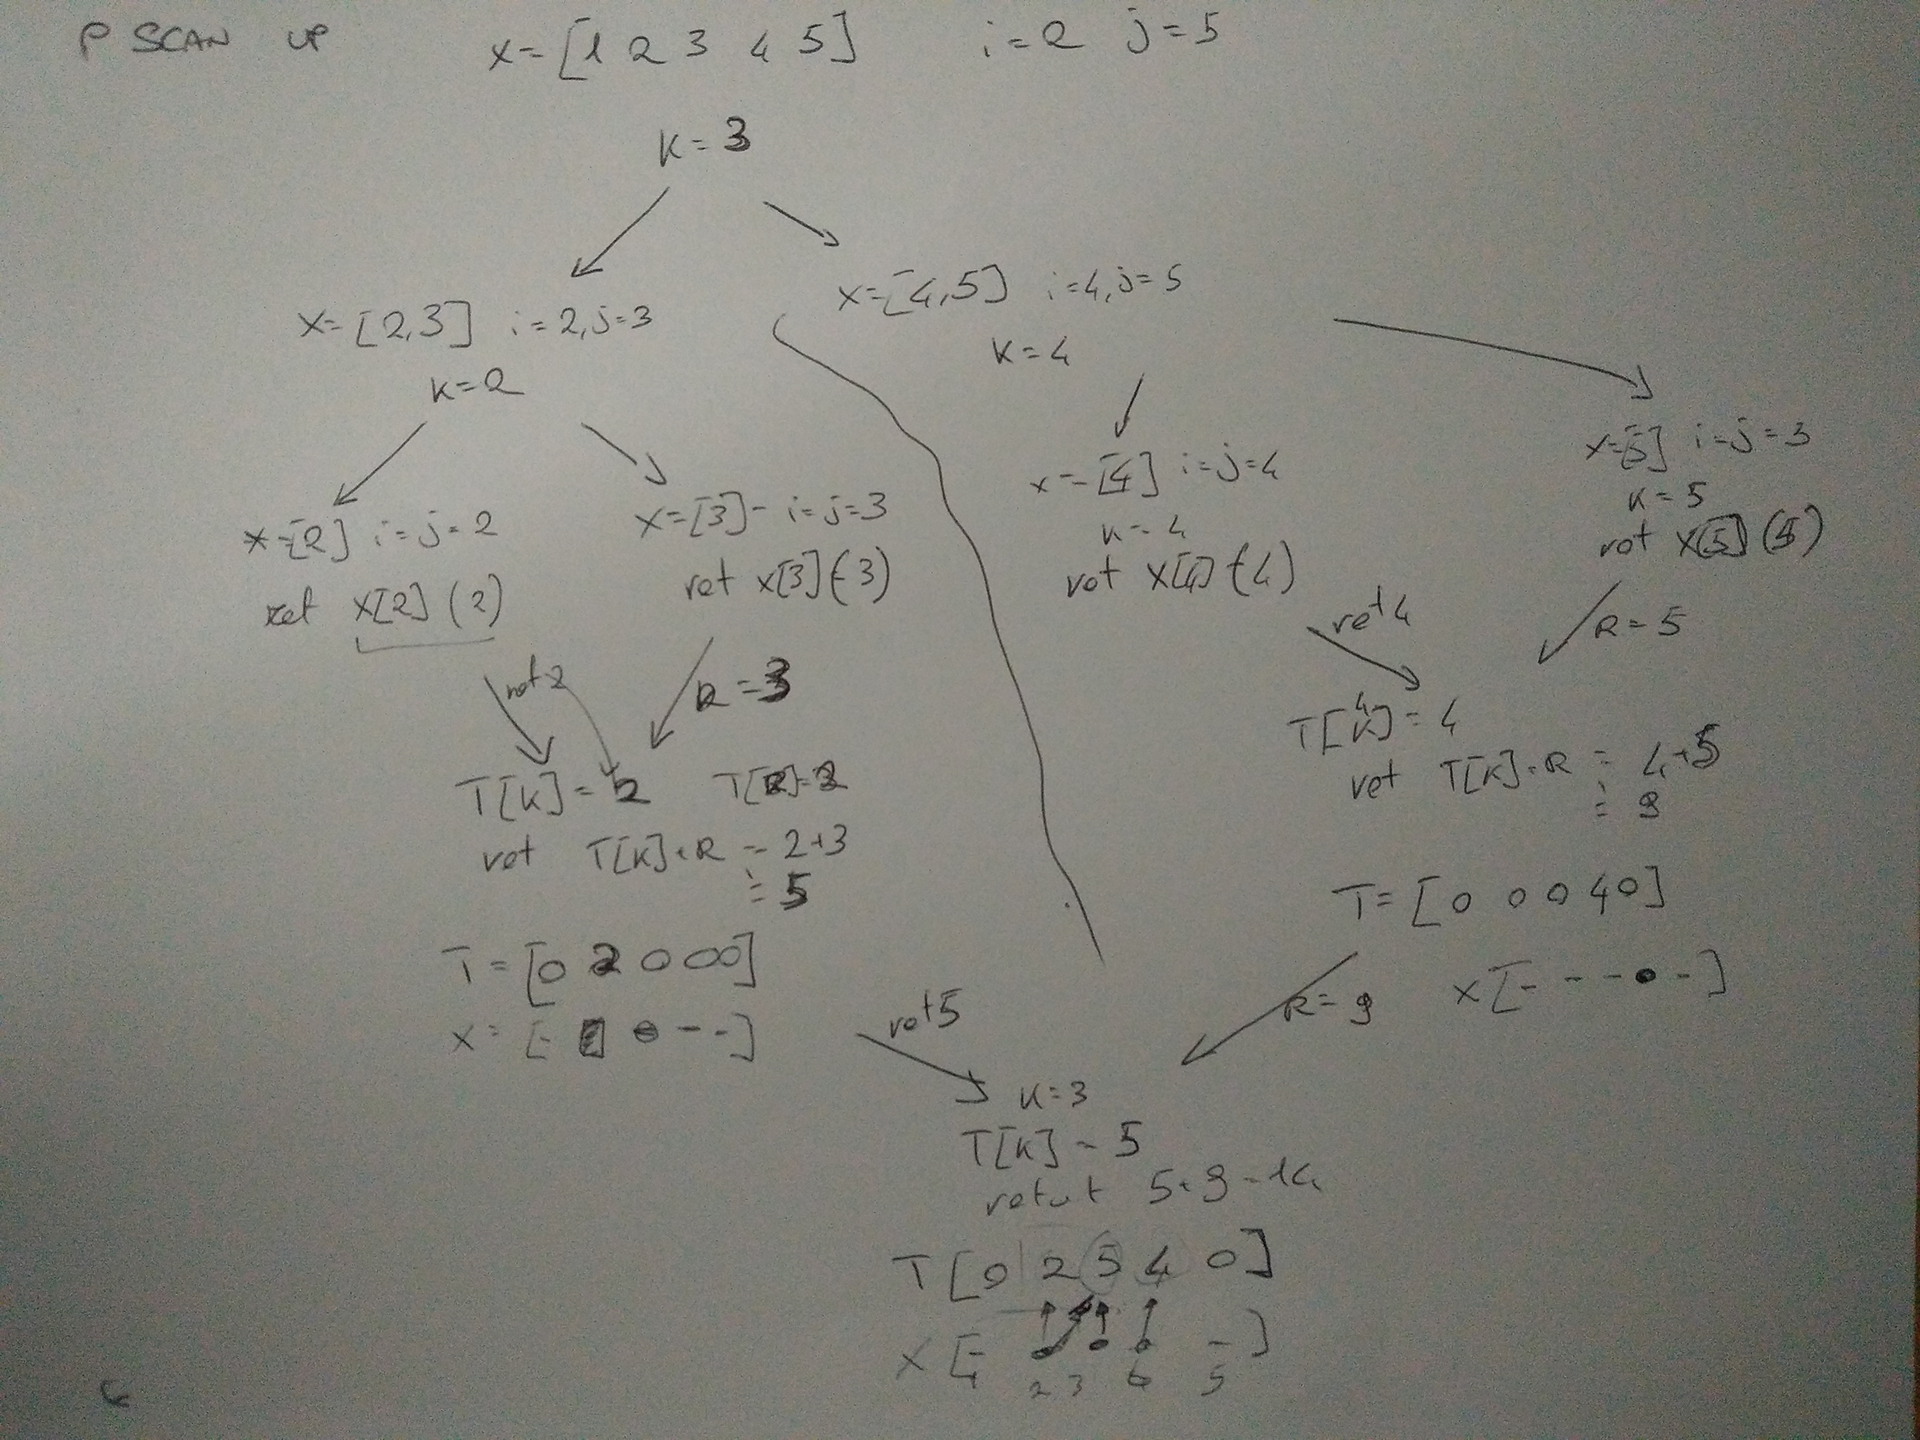
\includegraphics[width=\textwidth]{./notes/immagini/l27-pscanup.png}
	\caption{Albero delle chiamate per \textsc{P-Scan-Up}}
\end{figure}

La funzione \textsc{P-Scan-Down} utilizza le somme parziali prodotte da \textsc{P-Scan-Up} per calcolare e memorizzare nell'array \textit{y} i risultati finali.

Da notare che quando viene invocata la procedura per il calcolo dei valori a destra di $k$ viene utilizzato sia il valore \textit{v} della somma fino ad \textit{i} che il valore $T[k]$ che rappresenta la somma parziale dei valori della parte sinistra.

Anche in questo caso il nome della procedura indica la direzione in cui vengono effettuati i conti, ovvero durante la discesa dell'albero delle chiamate.

\begin{breakablealgorithm}
		\caption{\textsc{P-Scan-Down}}
		\begin{algorithmic}[1]
\Function{P-Scan-Down}{$v,x,t,y,i,j$}
    \State // $ v $ è il valore della somma fino ad $ i $ escluso
    \If{$i=j$}
        \State $y[i] \gets v+x[i]$
    \Else
        \State $ k \gets \lfloor(i+j)/2\rfloor$
        \State \textbf{spawn} \textsc{P-Scan-Down}($v,x,t,i,k$)
        \State \textsc{P-Scan-Down}($v+t[k],x,t,k+1,j$)
        \State \textbf{sync}
    \EndIf
\EndFunction
\end{algorithmic}
\end{breakablealgorithm}

\begin{figure}[htbp]
	\centering
	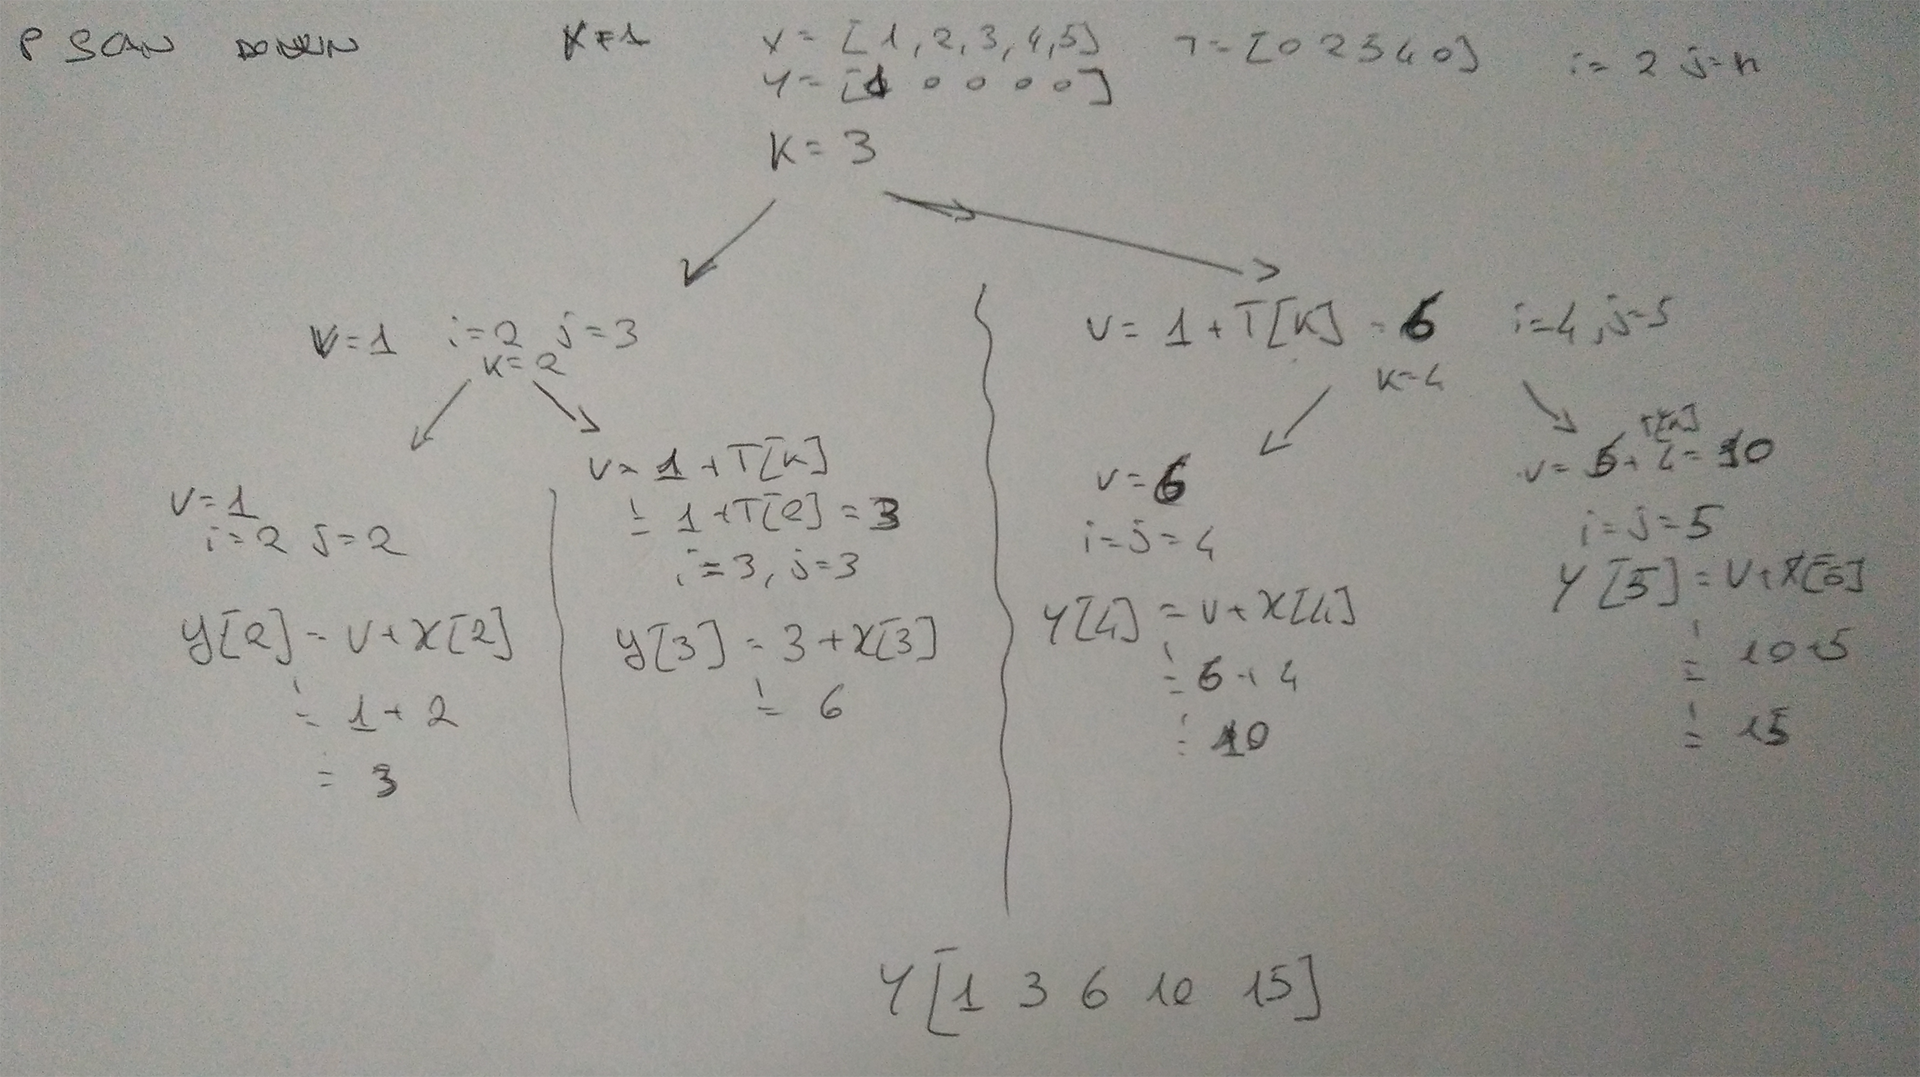
\includegraphics[width=\textwidth]{./notes/immagini/l27-pscandown.png}
	\caption{Albero delle chiamate per \textsc{P-Scan-Down}}
\end{figure}

Combinando le due procedure si ha quindi che le due chiamate parallele di entrambe le procedure lavorano sempre su dati distinti, evitando così delle race condition.

Il lavoro di \textsc{P-Scan} è

$$
T_{1}^{pscan}(n) = T_{1}^{pscan-up}(n) + T_{1}^{pscan-down}(n) + \Theta(1)
$$

e dal momento che anche le due chiamate vengono fatte in modo sequenziale, anche la durata è uguale a

$$
T_{\infty}^{pscan}(n) = T_{\infty}^{pscan-up}(n) + T_{\infty}^{pscan-down}(n) + \Theta(1)
$$

Sia \textsc{P-Scan-Up} che \textsc{P-Scan-Down} hanno la stessa durata e lo stesso lavoro, perché fanno operazioni molto simili, ci concentriamo quindi su \textsc{P-Scan-Up}, tanto la differenza è al più di una costante.

Tenendo a mente che $n = j - i +1 $

$$
T_{1}^{pscan-up}(n) = 2 T_{1}^{pscan-up}(n/2) + \Theta(1) = \Theta(n)
$$

e

$$
T_{\infty}^{pscan-up}(n) = T_{\infty}^{pscan-up}(n/2) + \Theta(1) = \Theta(\log n)
$$

Mettendo assieme i vari pezzi si ha che

$$
T_{1}^{pscan}(n) = 2 T_{1}^{pscan-up}(n) = \Theta(n)
$$

e

$$
T_{\infty}^{pscan}(n) = 2T_{\infty}^{pscan-up}(n) = \Theta(\log n)
$$

Il parallelismo dell'algoritmo risulta essere $\Theta(\frac{n}{\log n})$ che è molto buono.


\subsection{Correttezza dell'algoritmo}

Partiamo dalla funzione \textsc{P-Scan-Down}, la quale dato l'array di partenza e l'array di supporto contente le somme parziali delle varie parti sinistre, calcola nell'array finale il risultato.

La procedura riceve in input in valore \textit{v} con il risultato parziale degli elementi a sinistra della porzione dell'array sul quale viene invocata la procedura. La prima chiamata viene fatta utilizzando il valore in posizione 1, dato che entrambe le procedure iniziano a lavorare dal secondo elemento, perché il primo basta che venga semplicemente ricopiato.

Si ha quindi che se si verifica il caso base, ovvero la procedura viene invocata su un array con un solo elemento, viene effettuata la somma di \textit{v} con il corrispettivo elemento in input, la quale viene poi memorizzata nella corretta posizione dell'array con i risultati. Si ha quindi che il caso base gestito correttamente.

Nel caso ricorsivo, si ha che viene calcolata la posizione centrale dell'array sul quale si sta lavorando e viene invocata ricorsivamente la procedura sulla due parti destre e sinistre. Alla procedura che lavora sulla parte sinistra viene passato come valore di \textit{v} lo stesso ricevuto come parametro, ovvero la somma parziale dei valori che si trovano a sinistra della porzione dell'array sul quale si sta lavorando ed è il valore corretto perché la parte sinistra inizia alla stessa posizione della porzione corrente. Si ha quindi che la procedura ricorsiva sinistra viene invocata correttamente e su una porzione di array inferiore, quindi si può assumere induttivamente che vengano effettuate le operazioni corrette.

Per quando riguarda la parte destra, questa viene invocata con \textit{v} uguale a $v + T[k]$, ovvero la somma parziale della parte \textbf{a sinistra} della porzione corrente più la somma parziale della parte \textbf{sinistra} dell'array corrente e, assumendo che l'array \textit{T} sia stato calcolato correttamente, l'invocazione è corretta e quindi si può assumere induttivamente che vengano eseguiti i calcoli corretti.

Per quanto riguarda \textsc{P-Scan-Up}, si ha che, dato l'array dei valori, deve essere calcolato l'array $T$ contenente le somme parziali, in modo che 

$$
T\big[\lfloor n/2 \rfloor \big] = \sum\limits_{i=1}^{n/2} x[i]
$$

e deve ritornare la somma di tutti gli elementi della porzione dell'array di input che gli è stata fornita.

Nel caso base, con l'array contenente un solo elemento, si ha che il risultato parziale non viene calcolato perché la parte sinistra è vuota e viene ritornato il valore dell'unico elemento dell'array che è uguale alla somma di tutti gli elementi. Si ha quindi che il caso base viene gestito correttamente.

Nel caso ricorsivo, viene calcolato l'elemento mediano ed invocata ricorsivamente la funzione sulle due porzioni dell'array. Dal momento che le invocazioni vengono effettuate su una porzione ridotta dell'array, si può assumere che queste ritorno i valori corretti.
Si ha quindi che in $T[k]$ viene memorizzata la somma parziale della parte sinistra dell'array corrente, che è l'operazione corretta da fare, e che viene ritornato correttamente $T[k]+r$, ovvero la somma dei due parziali delle due parti, cioè la somma di tutti gli elementi dell'array d'invocazione.

Dato che entrambe le funzioni sono corrette, anche \text{P-Scan} è corretta.

\chapter{Geometria computazionale}

Ci sono varie applicazioni della geometria computazionale

Noi ci concentriamo sullo spazio bi-dimensionale.

L'elemento alla base di tutto è il punto, che sarà caratterizzato da due coordinate, le quali saranno tipicamente dei numeri float che sono soggetti a degli errori di arrotondamento.

Ma c'è sempre il piano B, ovvero utilizzare le coordinate intere a 32 bit.

Le nostre coordinate saranno quindi comprese tra un $-$\textsc{Maxint} e \textsc{Maxint}.

C'è però un problema, tipicamente nella geometria computazionale vengono calcolate delle aree, che devono anch'esse essere contenute in un intero e quindi i valori delle coordinate devono essere compresi in un intervallo $-$\textsc{CMax} e \textsc{CMax} con $\textsc{CMax} \leq \sqrt{\textsc{Maxint}} /2$, quindi facendo due conti si ha $\textsc{Maxint} = 2^{31} $ e $\textsc{CMax} = 2^{15}$.

E' poco ma sufficientemente buono, perché su uno schermo di un metro per un metro si ottengono 32 punti per ogni millimetro.

Una volta stabilito come rappresentare i punti si possono rappresentare:

\begin{itemize}
\item   un segmento, utilizzando due punti
\item   un cerchio, con il centro e il raggio
\item   un poligono, con una serie di punti che rappresentano i vertici.
\end{itemize}

Il vettore \emph{v} di coordinate $(v_x, v_y)$ viene rappresentato con uno qualsiasi dei segmenti orientati $\overrightarrow{pq}$ tali
che $v_x = x_q-x_p$ e $v_y = y_q - y_p$.

Talvolta con lo stesso simbolo può essere rappresentato sia il punto di coordinate $(x_p,y_p)$ che il \textbf{vettore posizione} $(x_p,y_p)$ rappresentato dal segmento orientato $\overrightarrow{op}$, dove \textit{o} è l'origine degli assi.

Il \textbf{prodotto vettoriale} di due vettori $v_1 = (x_1,y_1)$ e $v_2 = (x_2,y_2)$ è definito come l'area orientata del parallelogramma dato dai vertici: $o \equiv (0,0)$, $p_1 \equiv (x_1,y_1)$, $q \equiv  (x_1+x_2, y_1+y_2)$ e $p_2 \equiv (x_2, y_2)$.
L'orientamento è positivo se l'angolo da $v_1$ a $v_2$ è orientato in senso antiorario, con segno negativo altrimenti.

\begin{figure}
	\centering
	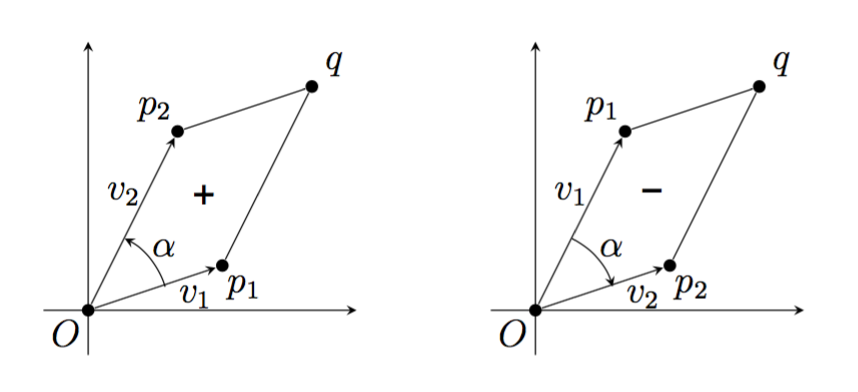
\includegraphics[width=0.7\textwidth]{./notes/immagini/l27-fig1.png}
	\caption{L'area orientata del parallelogramma individuato dai due vettori $v_1$ e $v_2$.}
\end{figure}

L'area orientata può essere calcolata come il determinate della matrice

$$
v_1 \times v_2 = \det \: \begin{bmatrix}
x_1 & x_2 \\
y_1 & y_2
\end{bmatrix} = x_1 y_2 - x_2 y_1
$$

questo perché l'area del trapezio è uguale a

$$
A = \frac{x_2y_2}{2} + x_1\frac{y_2+(y_1+y_2)}{2} - \frac{x_2y_2}{2} - x_2\frac{y_2+ (y_1+y_2)}{2} = x_1y_2 - x_2y_1
$$

Se cambio l'ordine dei punti, il segno dell'area cambia.
